\chapter{$K_S^0$ Reconstruction Study}

The final states of $B^0 \to K_S^0  K_S^0  K_S^0 $ only depends on the decay of $K_S^0$. The main decay channels of $K_S^0$ is to either $\pi^+ \pi^-$ at branching fraction of about 0.692, or to $\pi^0 \pi^0$ at branching fraction of 0.307, which are referenced from PDG\cite{pdg}.
 The characteristics of these two decays are much different in terms of the response from Belle II detector. The charged decay that yields  $\pi^+ \pi^-$ leaves two tracks originating from VXD or CDC volumes with opposite charges. On the other hand, the $\pi^0$ main decay channel is $\pi^0 \to \gamma \gamma$. This creates a bunch of clusters on ECL. The reconstruction of the decay channel is performed through  $\pi^+ \pi^-$. There are mainly two reasons for not selecting $\pi^0$ as final states.
 First, $\pi^0 \to \gamma \gamma$ can yield a large fraction of fake $K_S^0$. The reconstruction of two ECL clusters provides no constrain on $K_S^0$ vertex so it's almost impossible to suppress the combinatorial background using vertexing quality in this case. The only reliable selection will be the mass of $K_S^0$ which is typically distributed around its nominal mass with a few hundred of keV. 
 The $\gamma$ however, could be originating from many other resources, such as beam background and charged track radiation. Using mass window of $K_S^0$ could not effectively reject the noticeable fraction of fake $K_S^0$. Second, with $K_S^0$ reconstructed from neutral pions , the events of $B^0$ that consist of one or more such $K_S^0$ have poorly reconstructed vertices. To be noted that even with $B^0 \to K_S^0  K_S^0  K_S^0 $ which only uses $K_S^0$ from charged pions as the final states, there is no direct charged tracks from the interaction region, which leads to the worse resolution of vertex position compared to the channel like $B^0 \to J/\psi K_S^0$, which has two direct charged tracks of $e^+e^-$ or $\mu^+ \mu^-$ thanks to the very short flight distance of $J/\psi$. If one (or more) of $K^0_S$ has the poor vertexing quality from its decay products, it can further reduce the precision of vertex positions of $B^0$. This leads to a large uncertainties in defining the decay time of signal $B^0$ and the decay time difference. The latter is the key observable in TDCPV measurement. Based on above, only $K_S^0$ reconstructed using charged pions are considered in this analysis.
 
 \section{Cut-based $K_S^0$ Reconstruction}
 
 The $K_S^0$ has average life time at $(8.954 \pm 0.004) \times 10 ^{-11} \:\text{s}$. Therefore, the flight length of $K_S^0$ is comparable with the scale of detector size. In the typical Belle II energy scale, the flight length of $K_S^0$ is in a range from a few micrometer away from $B$ vertex, to more than 14 cm that is outside of the last layer of SVD ladder, see Figure \ref{ks_flight}.

 % check this plot for how to normalize
 \begin{figure}[htpb]
 	\centering 
 	\begin{minipage}[t]{0.45\linewidth}
 	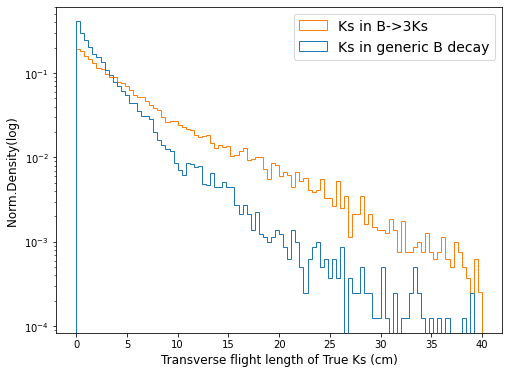
\includegraphics[width=0.9\linewidth]{ks_flight_XY}
 	\end{minipage}
	\begin{minipage}[t]{0.45\linewidth}
		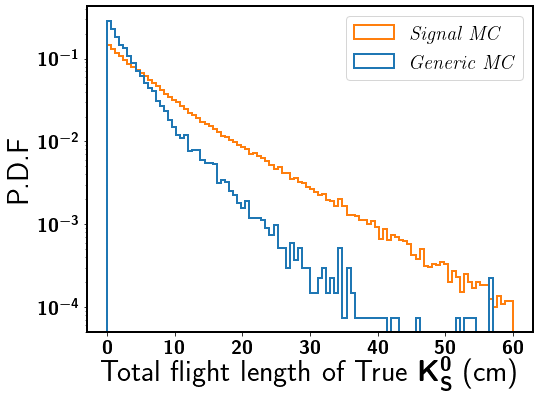
\includegraphics[width=0.9\linewidth]{ks_flight_All}
	\end{minipage}
 	\caption{The left is transverse flight length and the right is the total flight length from true $K_S^0$.  The blue is from generic MC and  the orange is from signal MC. It's clear that the average $K_S^0$ flight length in signal MC is longer. Both plots are normalized.}
 	\label{fig:ks_flight}
 \end{figure}
 
 Due to the different topology of $B^0$ decay, the average momentum of $K_S^0$ in generic MC is different from the ones from signal MC. While it's clear that the fraction of $K_S^0$ decaying outside the IP is the majority in both MC samples and therefore there's no reason to constrain $K_S^0$ decay vertices in IP. In general, the cut-based reconstruction for $K_S^0$ is first performed by the selection of invariant mass from its decay products. After the selection on invariant mass is applied, a vertex fit for each $K_S^0$ using charged pions' tracks is done without IP constraint. This reconstruction is mainly achieved by using standard BASF2 particle list called ``stdKshort:merged". In this ``stdKshort:merged" list, two $K_S^0$ particle collections are first reconstructed and then merged.
  
  We first take all the ``V0" objects from BASF2 Datastore which use 2 online reconstructed charged tracks with opposite charges and a converged fitted vertex. The invariant mass ``M" from two pions' 4-vector is calculated. The $K_S^0$ candidates with ``M" between $0.45 < M < 0.55$ GeV are selected, named ``Ks:V0". In addition to these $K_S^0$ from ``V0" objects, another $K_S^0$ collection from offline reconstruction is also formed. In this step, charged tracks with mass hypothesis of $\pi^{\pm}$ is used, which the tracks and PID of charged pions are pre-selected by the criteria in Table \ref{tab:kspipi_select}. Then $K_S^0$ are found by combining all of these tracks and the candidates with ``M" in between $0.3 \sim 0.7$ GeV before the vertex fit are kept. Then, vertex fit is perform for these candidates and the ones that have converged vertices and $0.45 < \text{M} < 0.55$ GeV are considered as the $K_S^0$ candidates, named ``Ks:reco", which uses the same criteria as ``V0"-based reconstruction. In both cases, the vertex fit is performed using ``TreeFit"\cite{krohn2020global} that is the recommended algorithm in Belle II. It's clear that there are duplication of $K_S^0$ if two collections are merged directly. Therefore, the objects' index of two daughters' tracks in the Datastore are compared between $K_S^0$ from these two collections, from which the identical combinations are removed to avoid duplication. 
  
  
   The $B^0$ reconstruction efficiency is highly sensitive to the efficiency of charged pions because the final states particles are three identical $K_S^0$ decaying to 6 charged pions. That's why only a very loose selection on $\pi^{\pm}$ is applied. The selected $K_S^0$ collection using cut-based method therefore contains many fake candidates, see the distribution of ``M" from cut-based selected $K_S^0$ from signal MC in Figure \ref{fig:ksM_sigmc}.
 
 
 \begin{table}[htbp]
 	\centering
 	\large
 	\caption{Pre-selection criteria of $\pi^+ \pi^-$ for $K_S^0$ offline reconstruction.}
 	\label{tab:kspipi_select}
 	\begin{tabular}{c c c c }
 		\toprule
 		Selection & $\theta$ & CDC Hits Number & PID  \\
 		\hline
 		Criteria  & CDC acceptance &  $>20$ & pionID $> 0.1$\\
 		\bottomrule
 	\end{tabular}
 \end{table}

% check y-axis and how many ks here.
\begin{figure}[htpb]
	\centering 
	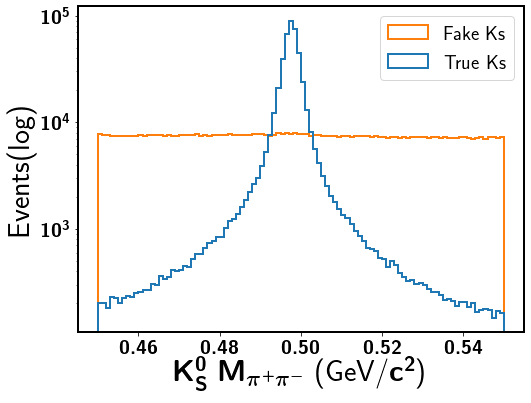
\includegraphics[width=0.7\linewidth]{Ks_M}
	\caption{``M" of $K_S^0$ from cut-based selection in signal MC (normalized). The blue line is the true $K_S^0$ and the orange is the fake $K_S^0$. }
	\label{fig:ksM_sigmc}
\end{figure}

The $K_S^0$ candidates from ``stdKshort:merged" is the default way to obtain $K_S^0$ in the current BASF2, 
however, the limitation of this cut-based $K_S^0$ reconstruction is the pollution from fake $K_S^0$. Using these $K_S^0$ candidates to reconstruct $B^0 \to K_S^0  K_S^0  K_S^0$, as long as one of three $K_S^0$ is fake, the reconstructed $B^0$ is fake, too. 
 This creates high fake rates in $B^0$ candidates and costs a large extra processing time for computing the kinematics and vertex fit of $B^0$ which should be avoided. Further, the number of combinatorial backgrounds in $B^0 \to K_S^0  K_S^0  K_S^0$ becomes high. It largely reduces the signal significance and introduce bias to the result of $\it{CP}$ parameters. Thus, a multi-variate analysis (MVA) based $K_S^0$ identification package, called ``KsFinder", is developed to further reject the fake $K_S^0$ from cut-based selected candidates.


% 2021.02.03 ends
\section{MVA-based $K_S^0$ Identification: KsFinder}

\subsection{Experience from Belle}
As mentioned in the last section, in order to improve the reconstruction performance of $K_S^0$ from cut-based selection, a MVA-based package called ``KsFinder" has been developed. The reconstruction of $K_S^0$ can be treated as a typical classification problem. The input is a set of observables that describes the characteristics of $K_S^0 \to \pi^+ \pi^-$ decay. The training  target is the true or fake flag from the MC truth-matching variable called ``isSignal" where isSignal = 1 (0) stands for being a true (fake) $K_S^0$. In the experience of Belle, the $K_S^0$ reconstruction was first done by using cut-based method to select primary candidates, then a MVA-based classifier was implemented by assigning two likelihood indicators to each $K_S^0$ candidates. The package used by Belle is called ``nisKsFinder"\cite{b2book} conventionally. It outputs the two likelihood variables based on ``NeuroBayes" algorithm\cite{feindt2006neurobayes}, which defines the goodness of $K_S^0$, called ``nb\_nolam" and ``nb\_vlike", respectively. As their names suggest, ``nb\_nolam" is the likelihood of not being a $\Lambda$ particle and ``nb\_vlike" is the likelihood of being a V0-like particle. A good $K_S^0$ candidate from ``nisKsFinder" is the one with a low likelihood of being $\Lambda$ particle and a high likelihood of being a V0-like particle, assuming the major backgrounds for $K_S^0$ is the mis-identified $\Lambda$ among V0-like particles. By putting cuts on these two variables, a purification of $K_S^0$ can be made, see Figure \ref{b1niskf}. It can effectively reduce fake $K_S^0$ from cut-based selected candidates, however, there are a few disadvantages about this method. First, ``NeuroBayes" is a commercial product that was developed over 10 years ago. The official support and update is stopped nowadays, so it's not an ideal method for an experiment like Belle II that has a quite long prospective in operation. Second, the classification is based on a joint cut on two variables, which might make the cut values hard to choose, for example, two different cuts might have very close purity. Last but not least, the classification of $K_S^0$ is not the directly targeted output of the neuro-network. Instead, it classifies the V0-like particle and ``$\Lambda$". Besides, the computation speed of this method is not very optimized compared to other popular methods in today's view. 

\begin{figure}[htpb]
	\centering 
	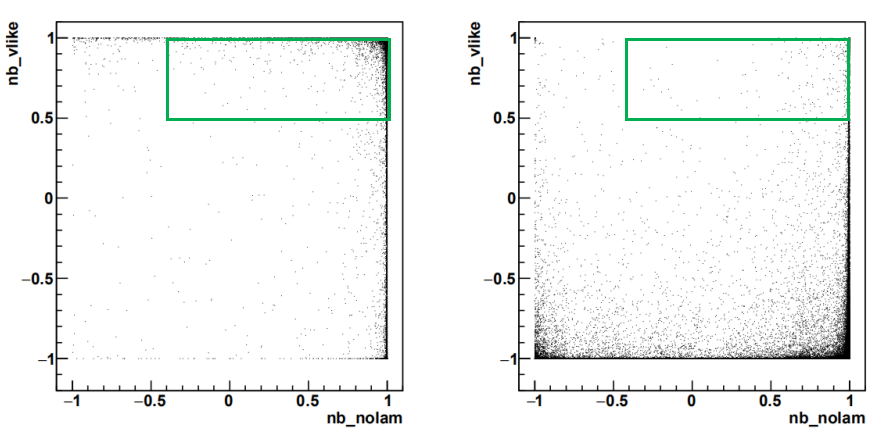
\includegraphics[width=0.7\linewidth]{nisksfinder}
	\caption{The distribution of two variables output from ``nisKsFinder": ``nb\_nolam" and ``nb\_vlike" for $K_S^0$ candidates from Belle signal MC. The left is from true $K_S^0$ and the right is from the fake $K_S^0$. In Belle, the standard cuts for $K_S^0$ is nb\_vlike $> 0.5$ and nb\_nolam $> -0.4$\cite{kang2020measurement}.}
	\label{b1niskf}
\end{figure}


In Belle II, such a dedicated $K_S^0$ classification tool is not implemented yet in BASF2 framework until 2019. Considered the limitation of Belle method, the development of $K_S^0$ classifier demands another algorithm and structure. The ``Boosted Decision Trees" (BDT) are widely employed for multivariate classification and regression tasks in modern high energy physics field. Particularly, a speed-optimized and cache-friendly
implementation of such method called FastBDT (FBDT) is popularly used\cite{keck2016fastbdt}. Compared to other popular classification algorithms such as TMVA, scikit-learn and XGBoost, FastBDT method is proven to be one order of magnitude faster during the training and applying phases\cite{keck2016fastbdt}. 


\subsection{FastBDT algorithm}
As the basic component of BDT, a general DT (decision tree) performs classification using a number of consecutive cuts at each tree nodes, where tree nodes are distributed on the layers of a tree. The maximum number of the layers is called ``depth of tree" and it's a hyper-parameter of a DT. Each data point contains labels (variables) called ``features" in DT. There are generally two phases in using DT for classification. One is ``training" (or ``fitting") phase that determines the best cut at each nodes. The other is called ``applying" phase that uses a trained DT to classifier a new data set. In training phase, training data points are fed to a DT and separated based on their features. At each node with a cut value, a cumulative probability histogram (CPH) can be defined by counting the signal and background data points. The histograms are used to determine the separation gain for a cut value at each position in these histograms. The feature and cut value (or
equivalently bin) with the highest separation power are used as the cut for the node. Hence, each cut value locally maximizes the separation gain between signal and background on the given
training sample. Eventually, on the last layer (called terminal layer), the signal fraction of all training data points in the same terminal node is used for the signal probability for a testing data point which ends up in the same terminal nodes, shown as Figure \ref{fig:DT}. In applying phase, a new data set, such as a test sample, is fed to the trained DT with fixed cut values at each nodes, to evaluate the performance of a DT or use it to separate the signal and background.

\begin{figure}[htpb]
	\centering 
	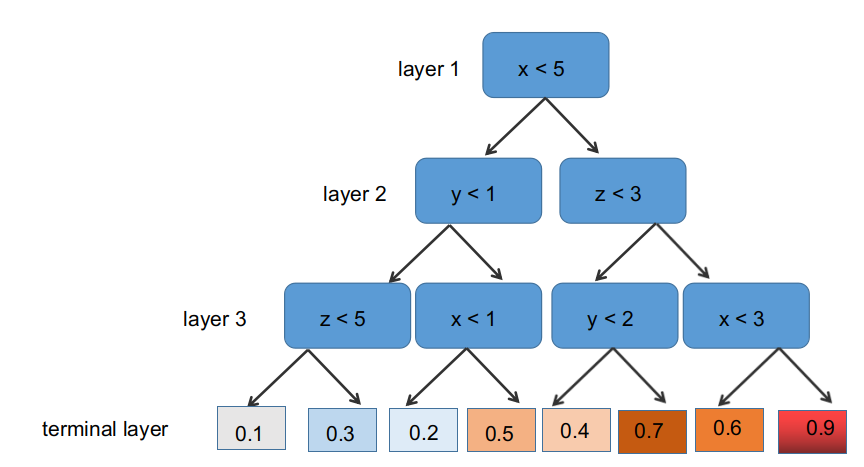
\includegraphics[width=0.7\linewidth]{DT}
	\caption{Basic structure of a DT with depth = 3 and labels (features) of x,y,z. The terminal layer contains training data points and are separated by cuts on layer 1 to 3. The number (color demonstrated) is the signal fraction of training data points in each terminal node, which is used for testing data points signal probability.}
	\label{fig:DT}
\end{figure}

The mathematical idea behind this method is to treat the data points as a data set defined on a multi-dimension hyper-space. As long as the signal/background data points show certain concentration in a sub-region of the hyper-space, it's possible to locally increase the signal fraction by consecutively cutting on the edge where signal and background are separated. The cut on labels at each node is the edge of the sub-region. A very deep DT (too many layers) means the edges of the sub-region of the hyper-space is cut too finely so that even small statistical fluctuation could be separated. Therefore, training data points in the sub-region can give a over-fitted signal fraction. As a result, the classifier is over-trained and performs poorly on new data points since the fluctuation is random in new data set. There are pruning algorithms which automatically remove cuts prone to over-training
from a DT, details can be found here \cite{olshen1984classification}.

Avoiding the over-training of a DT limits the depth of a tree strongly. For a problem of $K_S^0$ classification, the number of observables (features) is much more than the usual tree depth (a few layers). A single DT can only roughly separate the signal and background and thus, it's called a weak-learner. To improve the separation power, a sequence of many shallow DTs is formed during the training phase. For all the DTs, a negative binomial log-likelihood loss-function is minimized in the training phase. By using the results from many DTs (many weak learners), a well-regularized classifier with large separation power is constructed. The number of trees $N$ is called ``boosting steps", which is also the hyper-parameters for the training model. Such improved model is called ``Boosted Decision Trees" (BDT). There are a few different strategies to further optimize the performance of BDT such as ``Gradient Boost Decision Trees" (GBDT) and ``Stochastic Gradient Boost Decision Trees" (SGBDT) which use different methods to define the model output or increase the training speed, details are discussed here\cite{friedman2002stochastic}.


The FastBDT (FBDT) implements a optimized algorithm from a derived SGBDT method \cite{friedman2001greedy} and gain an order of magnitude faster execution time. FBDT reduces CPU time on CPH for tree nodes by using binned values for comparison to avoid  floating-point data calculation. It uses ``struct of arrays" that leads to a faster pre-cached CPU memory access pattern. The comprehensive comparison in terms of speed in fitting and applying phases between FastBDT and other popular methods such as XGBT, TMVA and scikit-learn is described in here\cite{keck2016fastbdt}. 

\begin{comment}
\begin{figure}[htpb]
\centering
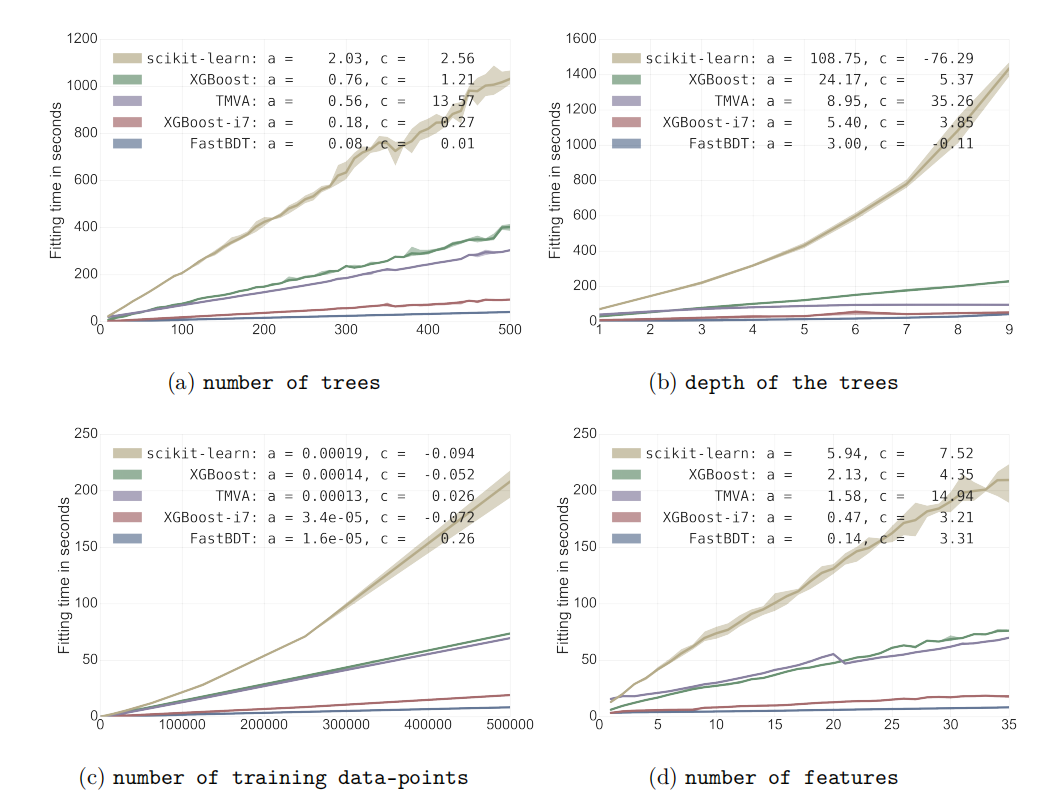
\includegraphics[height=12cm]{speedFBDT}
\caption{Runtime in fitting phase with different hyper-parameters comparison among FastBDT and XGBT,TMVA,scikit-learn.\cite{keck2016fastbdt}}
\end{figure}
\end{comment}

% 2021.02.04 ends
\subsection{Decay Topology of $K_S^0 \to \pi^+ \pi^-$}
The first step for developing $K_S^0$ MVA classification is to determine the input variables for FastBDT method which should represent the decay feature of $K_S^0$.
The remaining background of  $K_S^0 \to \pi^+ \pi^-$ after the cut-based reconstruction comes from different resources. In these resources, the main contributions are false combination of tracks, V0-like particle mis-identification, and looped tracks. 

The false combination of tracks includes two major cases. First is when one of the two daughter is $\pi^{+/-}$ and the other is not. This often happens when a charged pions from a neutral mother with a capability of decaying into multiple charged tracks, like $D^+ \to \mu^- \nu_{\mu} K^- \pi^+$. On the other hand, it's also possible that both of two tracks are correctly reconstructed from $\pi^{+/-}$ but they are not from the same mother, or the mother is not a $K_S^0$ particle due to the missing of other daughters, such as $D^+ \to K_S^0 (  \to \pi^+ \pi^-) \pi^+$. The decay shape resembled the above cases are illustrated as the following:  


\begin{figure}[htpb]
	\begin{minipage}[t]{0.5\linewidth} % 如果一行放2个图,用0.5,如果3个图,用0.33
		\centering 
		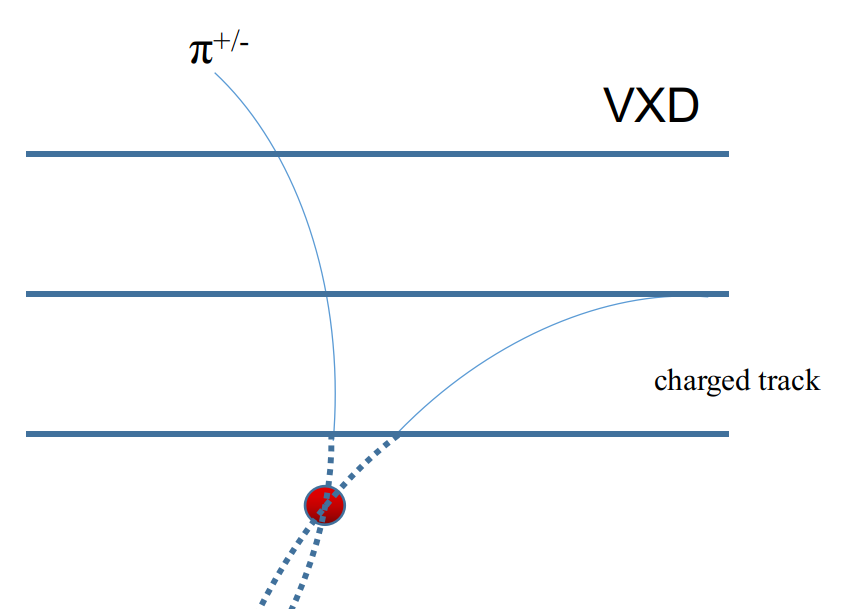
\includegraphics[width=7cm]{fakeks1} 
		\label{fig:side:a} 
	\end{minipage}%
	\begin{minipage}[t]{0.5\linewidth} 
		\centering 
		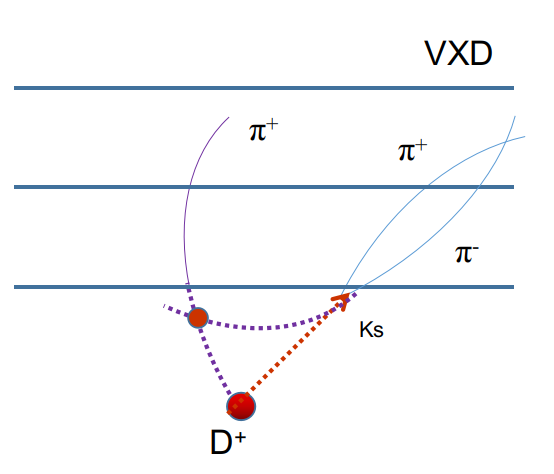
\includegraphics[width=7cm]{fakeks2} 
		%\caption{ } 
		\label{fig:side:b} 
	\end{minipage}% 
	
	\caption{The left shows the case when a charged track (not a pion) combined with a true pion as a fake $K_S^0$, the right shows the case when two daughters are correctly reconstructed as pion but not from the correct mother. }
\end{figure}

The V0-like particles mainly refer to $K_S^0$, $\Lambda$ and $\gamma$. $\gamma \to e^+ e^-$ yield is significantly lower than the previous two types and the mass different between pion and electron is very large, so the PID values can be used to well-distinguished them. As for the contribution of $\Lambda \to p^+ \pi^-$, it's happens when the positive charged tracks (proton track) is wrongly identified as $\pi^+$, see Fig 3-6 left. The key observable to distinguish this background is the invariant mass of mother particle, which $\Lambda$ is at 1.115 GeV, much larger than the $K_S^0$. The left-over $\Lambda$ after the cut-based reconstruction is minimal and can be further reduced by checking the PID information of the positive charged daughter. 

When a charged pion only carries a minimal of its mother's transverse momentum $p_T$, the curvature of its track may form a self-loop of which radius is comparable with the size of Belle II detector (mainly VXD and CDC) in $r-\phi$ plane. In this case, one charge pion could leave two charged tracks candidates with the opposite charge and similar $p_T$, with a possibility to form a converged vertex. Thus it also gives a potential fake $K_S^0$, see Fig 3-6 right.

\begin{figure}[htbp]
	\begin{minipage}[t]{0.5\linewidth} % 如果一行放2个图,用0.5,如果3个图,用0.33
		\centering 
		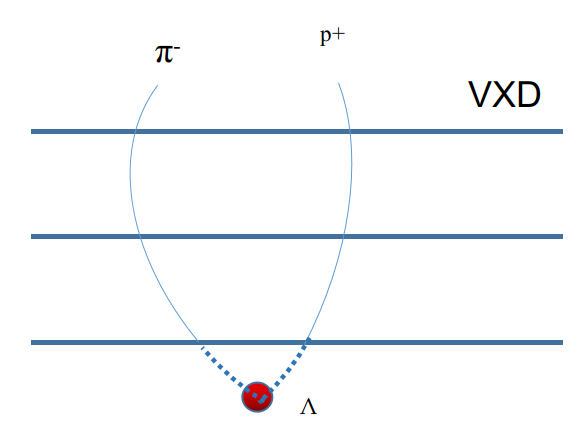
\includegraphics[width=7cm]{fakeks3} 
		\label{fig:side:a} 
	\end{minipage}%
	\begin{minipage}[t]{0.5\linewidth} 
		\centering 
		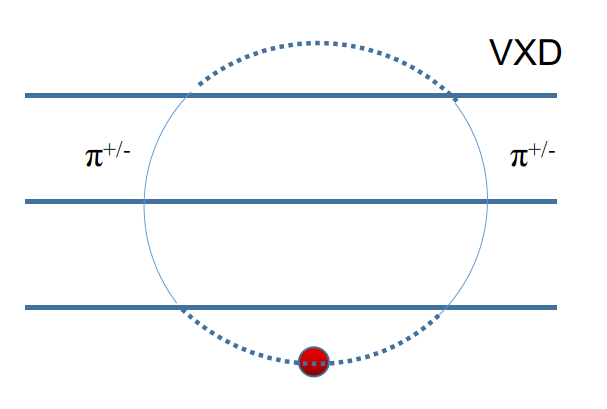
\includegraphics[width=7cm]{fakeks4} 
		%\caption{ } 
		\label{fig:side:b} 
	\end{minipage}% 
	
	\caption{The left shows the $\Lambda \to p^+ \pi^-$ decay shape that can be treated as $K_S^0$, the right shows a self-loop formed by a low $p_T$ charged pion reconstructed as two separated tracks with a vertex}
\end{figure}

\subsection{Determination of training observables from $K_S^0$ decay }
Given the characteristics of  $K_S^0 \to \pi^+ \pi^-$ discussed in the previous section, a set of observables as training features of FastBDT classifier can be constructed. The set includes categories of observables: kinematics, decay shape parameters , particle identifications and detector hits information. Observables are listed below with a sketch showing the shape parameters of $K_S^0$ decay in Fig 3-8. 

\begin{itemize}
	\item Kinematics
	\begin{itemize}
		\item Invariant mass of $K_S^0$ before and after fitting vertex
		\item momentum of $K_S^0$ and $\pi^{+/-}$, vectors and magnitudes. 
	\end{itemize}
	
	\item Decay shape parameters
	\begin{itemize}
		\item cosine angle between $K_S^0$ vertex and momentum.
		\item helicity angle of two daughters in reference of $K_S^0$ momentum.
		\item decay angle of two daughters in the mother's frame. 
		\item flight distance projection on $K_S^0$ momentum direction.
		\item significance of flight distance, defined by ratio of flight length and its uncertainties.
		\item distance on z-axis of two daughters helix 
		\item impact parameters on $K_S^0$ vertex
	\end{itemize}
	
	\item Particle identifications
	\begin{itemize}
		\item pion-ID for $K_S^0$ daughters.
		\item muon-ID for $K_S^0$ daughters.
		\item proton-ID for $K_S^0$ positive charged daughter. 
	\end{itemize}

	\item Hits information
	\begin{itemize}
		\item the number of PXD hits for each $K_S^0$ daughter, up to 2.
		\item the number of SVD hits for each $K_S^0$ daughter.
		%\item the number of CDC hits for each $K_S^0$ daughter. 
	\end{itemize}
	
\end{itemize}

\begin{figure}
	\centering
	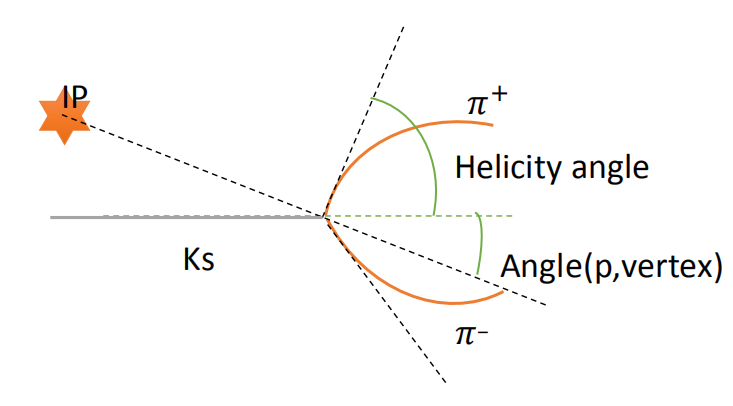
\includegraphics[height=6cm]{decayshape}
	\caption{The decay shape parameters, vertex vector takes IP as origin. }
\end{figure}


The decay shape category is of the most importance because it demonstrates the best separation power. For instance, if a false combination is made of two tracks, it's likely that the momentum direction of reconstructed fake $K_S^0$ is not aligned with the vertex position. So the projection of flight length on the momentum could be negative value for background. While in case of a true $K_S^0$, such projection is almost always a positive value.
 
There are a few points to be checked for using FastBDT classification, given the nature of the algorithm.
 First, the distribution of the observables should be different in true $K_S^0$ and background, so the FastBDT classifier can perform distinguish the true and the fake at each nodes to maximize the separation gain, just as Section 3.2.2 discussed. Secondly, there will a correlation among the training observables and they should also be different in signal and background. The boosting phase will create a sequence of shallow DTs whose structures are not same. Different correlations helps improve the performance of DTs in tuning of structure. For instance, a true $K_S^0$ flights longer by larger momentum in general, so its daughters' detector hits number becomes fewer. Then these two observables have negative correlations in true $K_S^0$. In case a fake $K_S^0$, the flight length could be a deep outside of VXD  but daughters may have full VXD hits, without clear correlation. At last, one should also avoid using many observables with too strong correlations since the classifier won't gain much improved separation power when put a cut on each of them. The correlation of the observables in signal and background samples are shown in Fig 3-9. The selected observables meets the requirements for classification. 
 
 \begin{figure}
 	\centering 
 	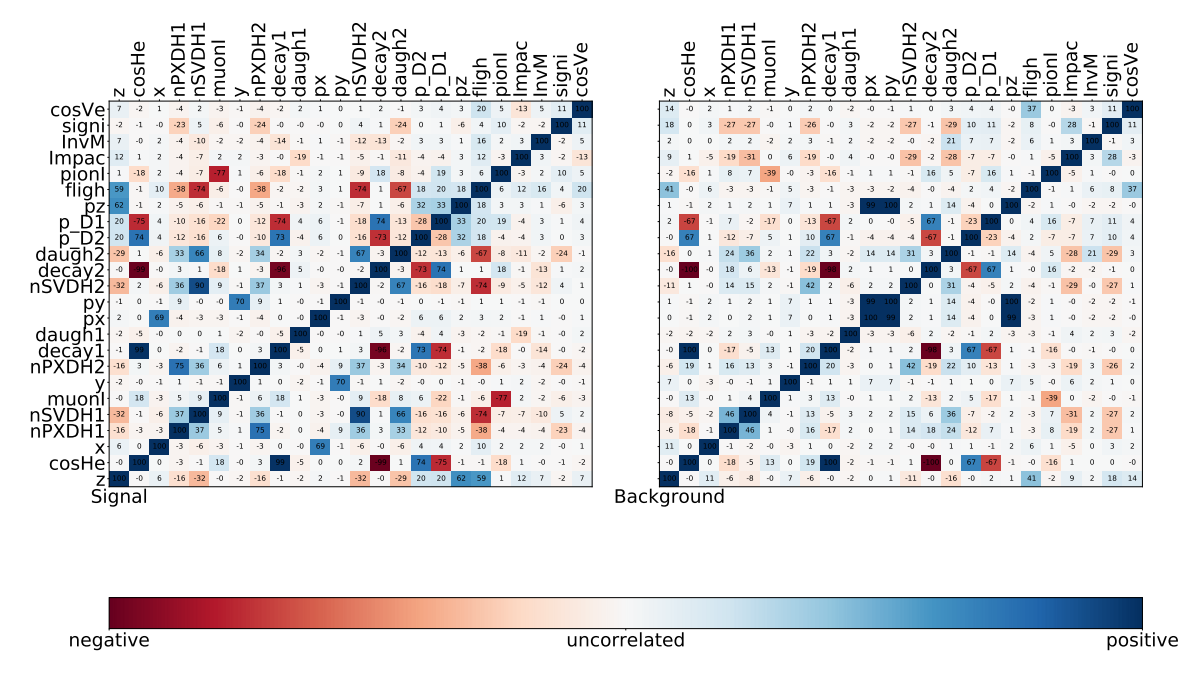
\includegraphics[height=8cm]{corks}
 	\caption{The correlation matrix of the chosen observables. It shows different correlation between observables in signal and background. And there's no single observable showing strong correlation with all other members. }
 \end{figure}
 

 \subsection{Training, Testing and Application of KsFinder}
 Training samples of $K_S^0$ are first extracted based on ``stdKshort:merged" from generic $B^0$ decay and $B^0 \to K_S^0  K_S^0  K_S^0$ using MC13 samples, respectively. For the hyper-[arameters of FastBDT method, the depth of each DT is 3 and the number of total trees (boosting steps) is 200, with a balance of computing time and performance. The training target variable is ``isSignal" flag. The ratio between the true and fake $K_S^0$ is 1:1 in both training and tesing sample. The training sample and tesing sample are separately prepared using different input file from MC13. The distribution of observables in true and fake samples (from $B^0 \to K_S^0  K_S^0  K_S^0$) are shown in the Appendix A. The abbreviations of those variables and their importance rank are shown in Table 3.2 and 3.3. 
 
 \begin{table} [ht]
 	\begin{minipage}[t]{0.5\linewidth}
 		\centering
 		\caption{The Abbreviations.}
 		\begin{tabular}{c|c}
 			\hline
 			Observables &  Abbreviations\\
 			\hline
 			nPXDHits\_D1 &  nPXDH1 \\
 			decayAngle\_D1 & decay1 \\
 			nPXDHits\_D2 & nPXDH2\\
 			y & y \\
 			decayAngle\_D2 & decay2\\
 			px & px\\
 			z & z \\
 			cosHelicityAngleMomentum & cosHe\\
 			x & x \\
 			daughtersDeltaZ & daugh1\\
 			nSVDHits\_D1 & nSVDH1\\
 			py & py\\
 			muonID\_pi & muonI\\
 			nSVDHits\_D2 & nSVDH2\\
 			p\_D1 & p\_D1\\
 			p\_D2 & p\_D2\\
 			pz & pz \\
 			flightDistance & fligh\\
 			pionID\_pi & pionI\\
 			InvM & InvM \\
 			daughterAngle2body & daugh2\\
 			ImpactXY & Impac \\
 			significanceOfDistance & signi \\
 			M & M \\
 			cosVertexMomentum & cosVe \\
 			\hline
 		\end{tabular}
 		\label{fig:side:a} 
 	\end{minipage}
 	\begin{minipage}[t]{0.5\linewidth}
 		\centering 
 		\caption{Importance rank }
 		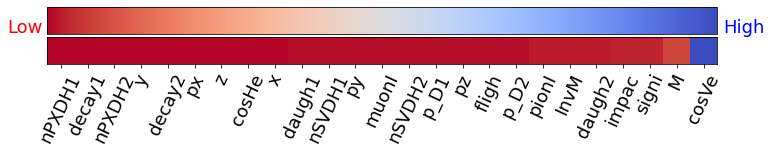
\includegraphics[width=4cm]{rank1}
 		\label{fig:side:b} 
 	\end{minipage}
 \end{table}

\subsection{The Performance and Over-fitting check}
The performance of classifier is evaluated by applying it on a independent data sample. So in the accordance of training data used, the same mount of events are prepared. Since the training is performed on three different types samples, three classifiers are actually obtained. Signal efficiency and background rejection are calculated using the output of trained classifier that presents the likelihood of probability of being a true $K_S^0$, as defined in Eq (3.1) and Eq (3.2).  

\begin{eqnarray}
	\text{signal efficency} = \frac{\text{Number of true $K_S^0$ with output $>$ cut value}}{\text{Number of all true $K_S^0$ }} \\
	\text{background rejection} = \frac{\text{Number of fake $K_S^0$ with output $<$ cut value}}{\text{Number of fake true $K_S^0$ }}
\end{eqnarray}

Using the weight file created by the training process, the output between 0 and 1 is assigned to every candidates as a quality index standing for the likelihood to be true $K_S^0$ that can be used as a cut. In order to check the performance of the classification, the ROC (receiver operating characteristics) curve is plotted, which shows the dependence of rejection power regarding the signal purity. The larger area a ROC curve is covered, meaning that background rejection drops slower when increasing classifier cut, the better performance is achieved. Three classifiers are tested with generic $B^0$ decay, and $B^0 \to K_S^0  K_S^0  K_S^0$ to check the robustness of classifier. The ROC, signal efficiency and purity are shown: 

\begin{figure}[H]
	\begin{minipage}[b]{0.5\linewidth}
		\centering 
		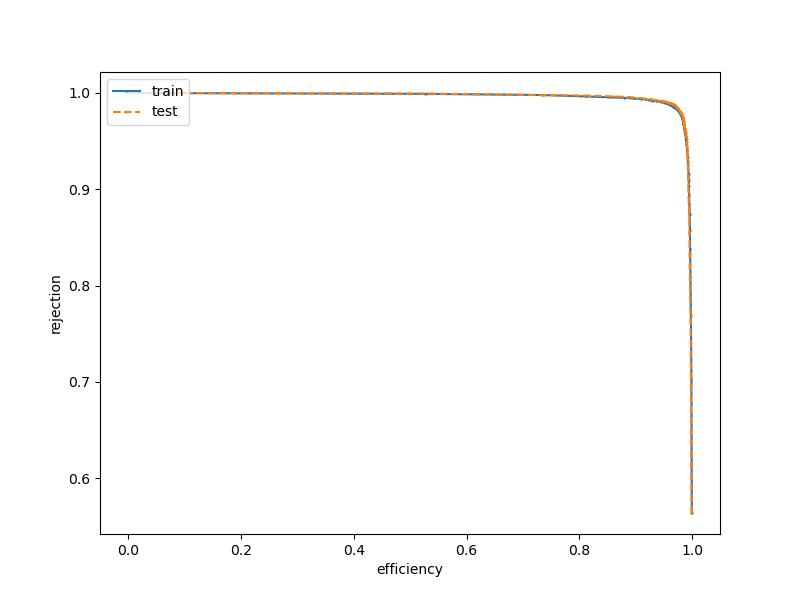
\includegraphics[height=6cm]{ROC_3Ks}
		\label{fig:side:a}
	\end{minipage}
	\begin{minipage}[b]{0.5\linewidth}
		\centering 
		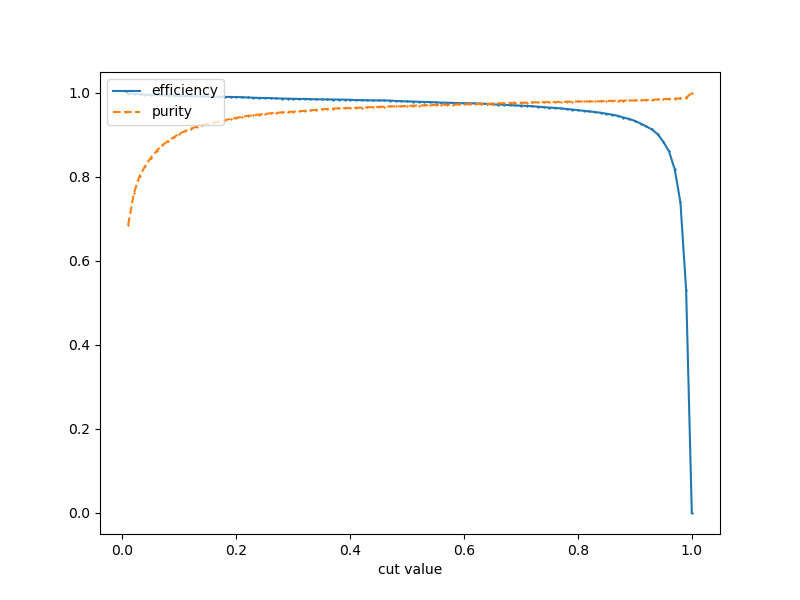
\includegraphics[height=6cm]{eff_3Ks}
		\label{fig:side:b}
	\end{minipage}
\caption{The left is ROC curve(blue for training and orange for testing) and the right is efficiency and purity (blue for efficiency and orange for purity) depending on cut of classifier output. Results are from $B^0 \to K_S^0  K_S^0  K_S^0$ sample.}
\end{figure}

\begin{figure}[H]
	\begin{minipage}[b]{0.5\linewidth}
		\centering 
		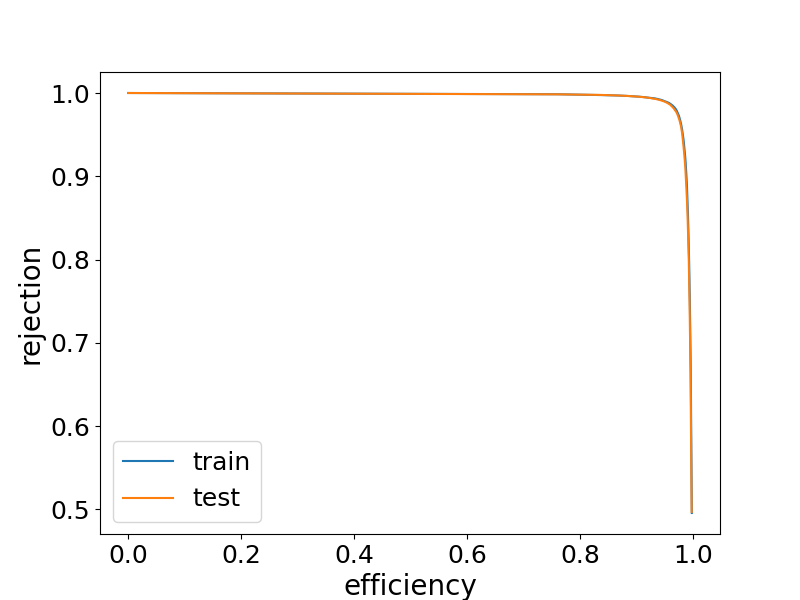
\includegraphics[height=6cm]{ROC_gen}
		\label{fig:side:a}
	\end{minipage}
	\begin{minipage}[b]{0.5\linewidth}
		\centering 
		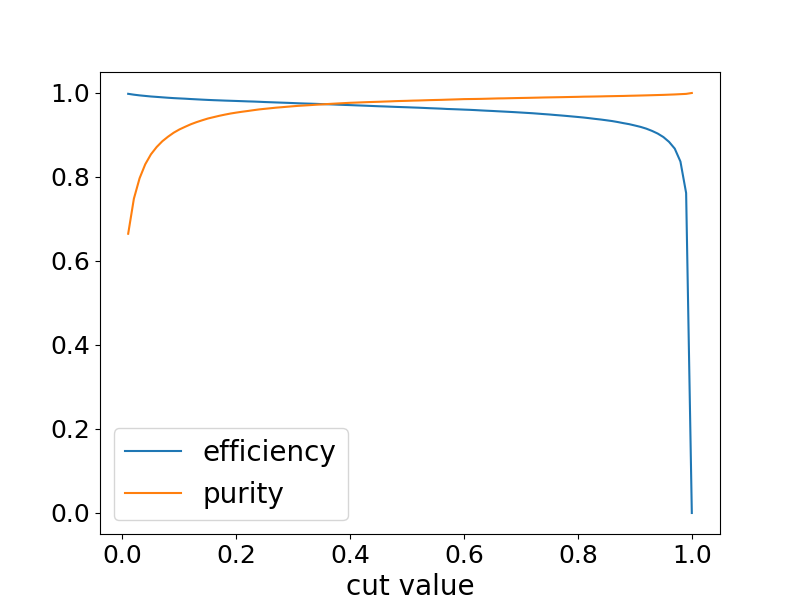
\includegraphics[height=6cm]{eff_gen}
		\label{fig:side:b}
	\end{minipage}
	\caption{The left is ROC curve (blue for training and orange for testing) and the right is efficiency and purity (blue for efficiency and orange for purity) depending on cut of classifier output. Results are from $B^0$ generic decay sample.}
\end{figure}

\begin{comment}
\begin{figure}[H]
	\begin{minipage}[b]{0.5\linewidth}
		\centering 
		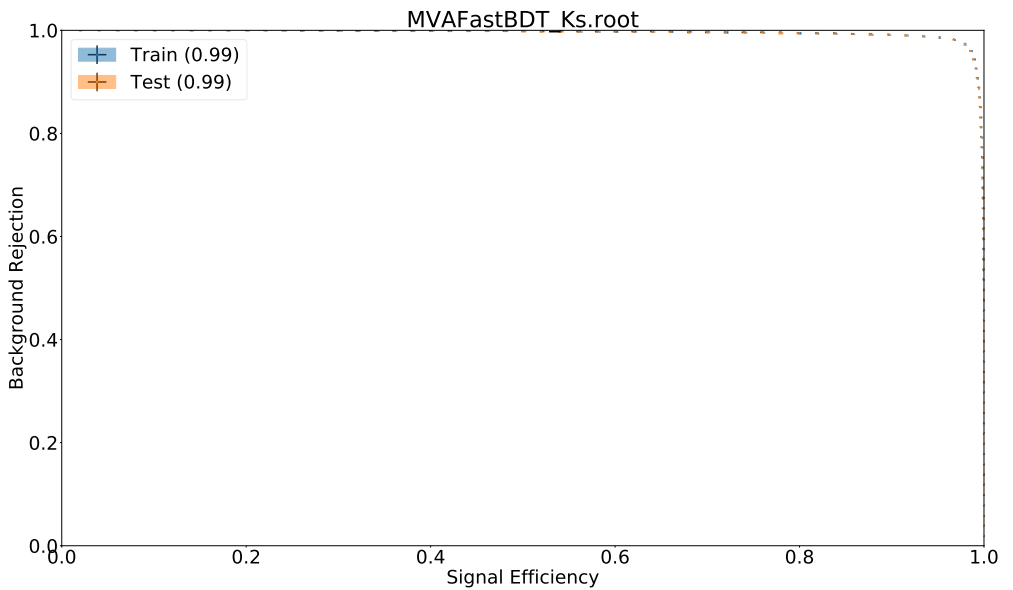
\includegraphics[height=4cm]{jpsi-jpsi}
		\label{fig:side:a}
	\end{minipage}
	\begin{minipage}[b]{0.5\linewidth}
		\centering 
		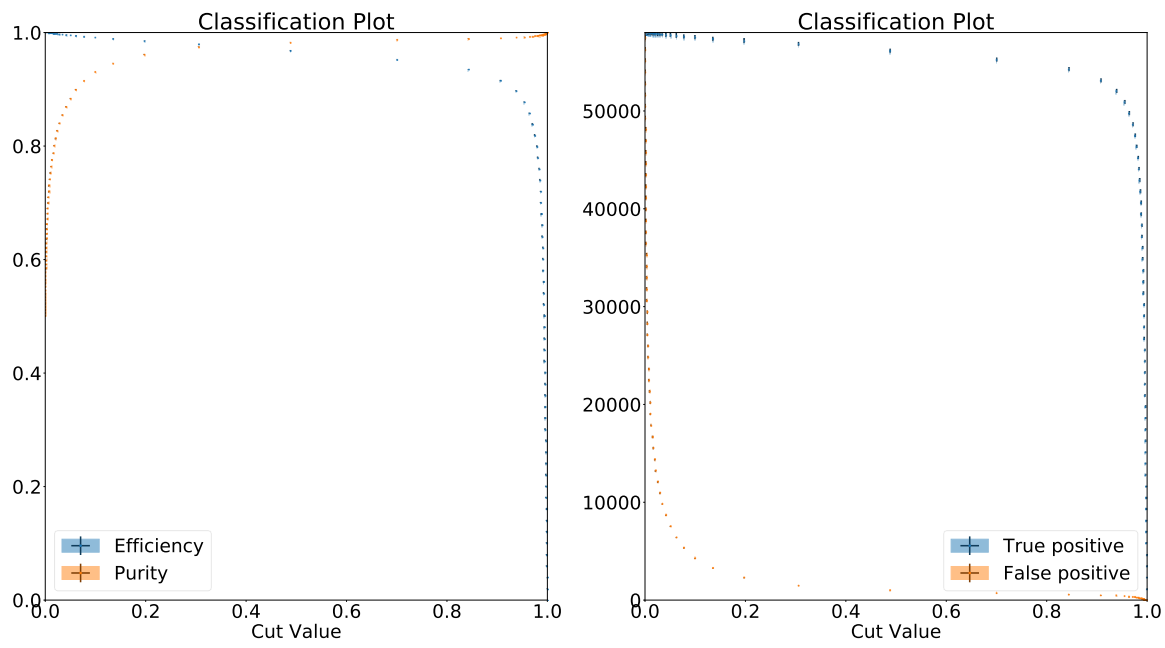
\includegraphics[height=4cm]{jpsi-jpsi-pur}
		\label{fig:side:b}
	\end{minipage}
	\caption{The left is ROC curve and the right is efficiency and purity depending on cut of classifier output. Results are from $B^0 \to J/\psi K_S^0$ generic decay sample.}
\end{figure}
\end{comment}


The ROC curves show a good rejection power on classifiers. To be noted, the curves are consistent in training and testing samples. 
While the ROC curve has shown the absence of noticeable over-fitting in classification, the detailed check can be made by comparing the distribution of classifier output on true and fake $K_S^0$ respectively in training and testing. In the classifiers we obtained, results from training and testing are very much close thus no over-fitting is spotted, as shown in Fig 3-13.
\begin{figure}[H]
	\begin{subfigure}{1\linewidth}
		\centering
		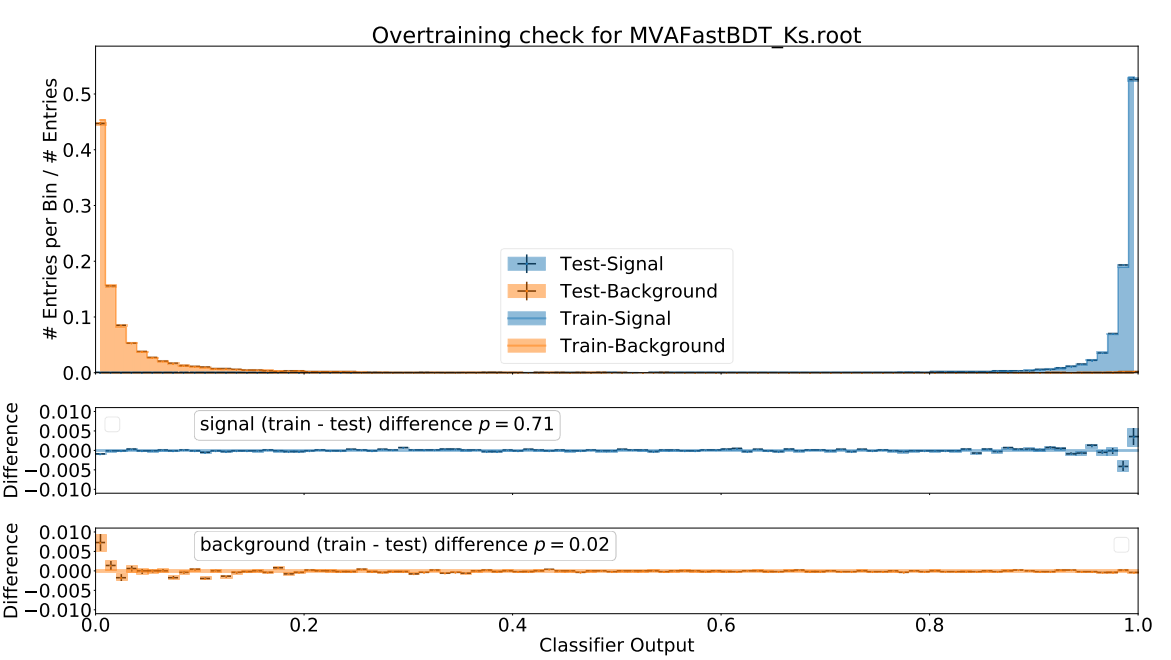
\includegraphics[height=6cm]{over-3ks}
		\caption{Over-fitting check for $B^0 \to K_S^0  K_S^0  K_S^0$.}
	\end{subfigure}
  	\vspace{0.3cm}

	\begin{subfigure}{1\linewidth}
		\centering
		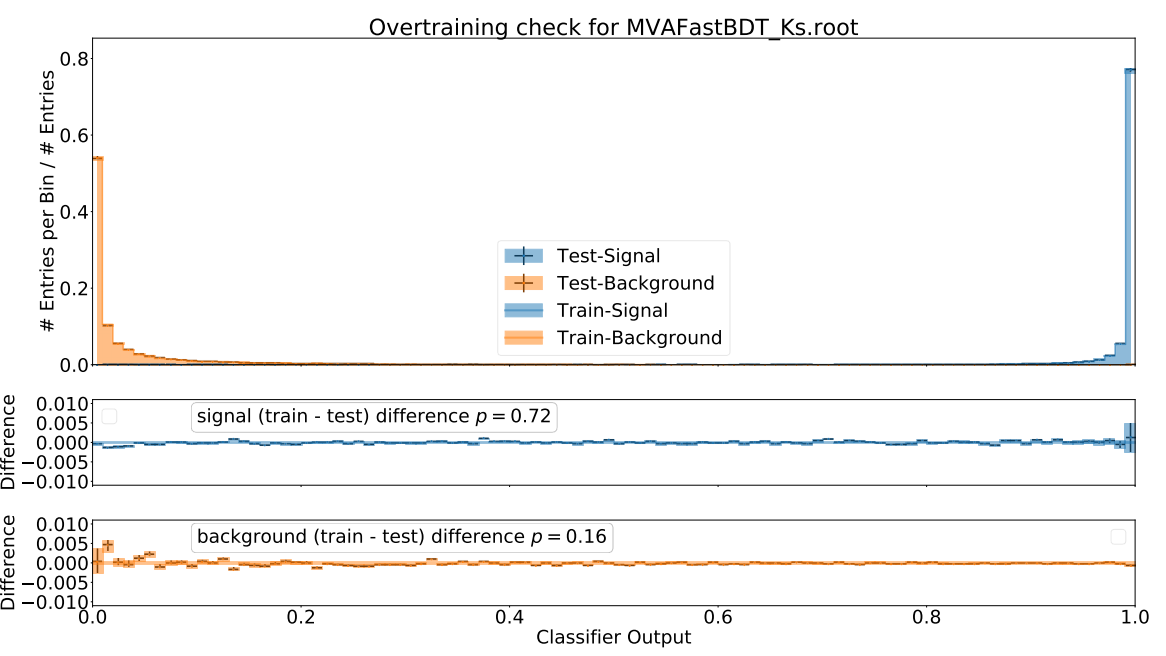
\includegraphics[height=6cm]{over-gen}
		\caption{Over-fitting check for $B^0$ generic decay.}
	\end{subfigure}
	\vspace{0.3cm}
	
%	\begin{subfigure}{1\linewidth}
%		\centering
%		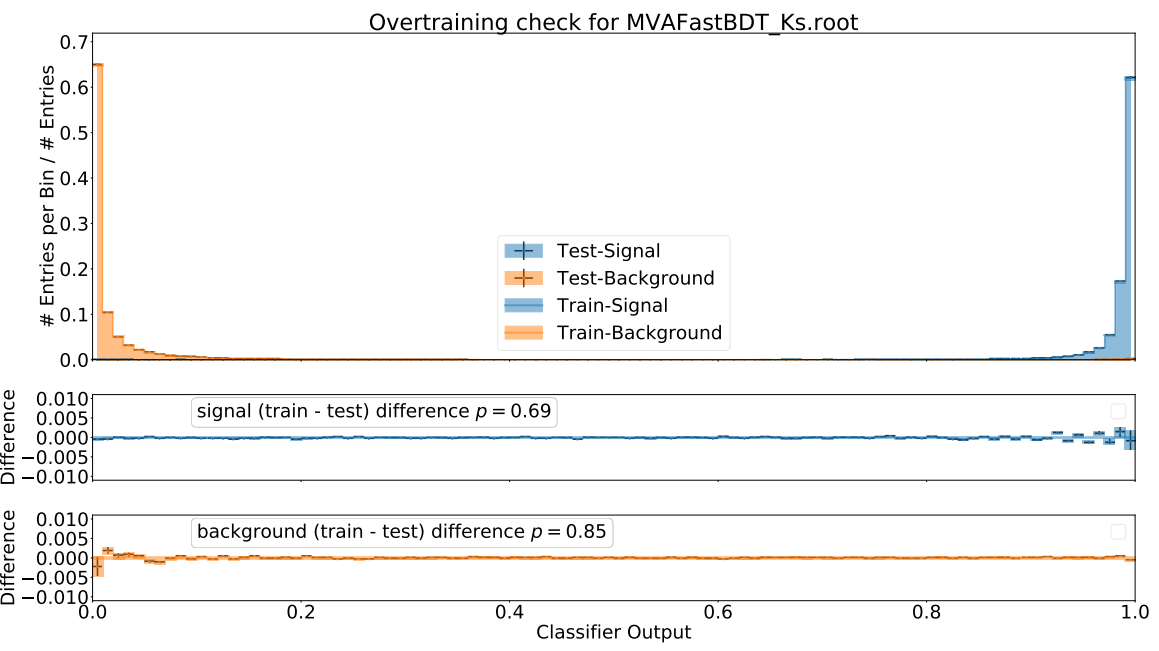
\includegraphics[height=6cm]{over-jpsi}
%		\caption{Over-fitting check for  $B^0 \to J/\psi K_S^0$.}
%	\end{subfigure}
%\caption{Over-fitting check for classifiers.}
\end{figure}

In order to use the output of KsFinder, a cut value must be chosen. The output of KsFinder is named ``FBDT\_Ks". Here we can define a ``Figure of Merit" (FOM) to determine the cut value. S and B is the number of true and fake $K_S^0$ after the cut,respectively. The value of 0.74 of ``FBDT\_Ks" maximize the KsFinder output in $B^0 \to K_S^0  K_S^0  K_S^0$, so we will use this value as only $K_S^0$ with larger ``FBDT\_Ks" will be kept from cut-based selection.

\begin{equation}
	\text{FOM} = \frac{S}{\sqrt{S+B}}
\end{equation}

\begin{figure}[H]
	\centering
	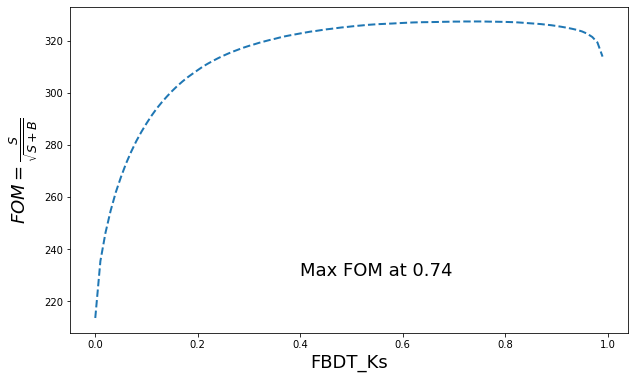
\includegraphics[width=0.6\linewidth]{fom3ks}
	\caption{FOM of classifier output (FBDT\_Ks) in $B^0 \to K_S^0  K_S^0  K_S^0$, maximum value is obtained at 0.74 and curve is almost flat after 0.5.}
\end{figure}

By comparing the fitted invariant mass of $K_S^0$ before and after the application of this cut, it's clear that the fraction of background has been largely reduced and most of the signal remains. The true $K_S^0$ fraction in the pre-selected $K_S^0$ before applying KsFinder cut is 39\%, and 95.3\% of them are remained after KsFinder applied. The fake $K_S^0$ fraction before applying KsFinder cut is 61\%, and 97.6\% of them are rejected after KsFinder applied. A much cleaner $K_S^0$ candidates is created as shown in Fig 3-15. 

\begin{figure}[htpb]
	\centering
	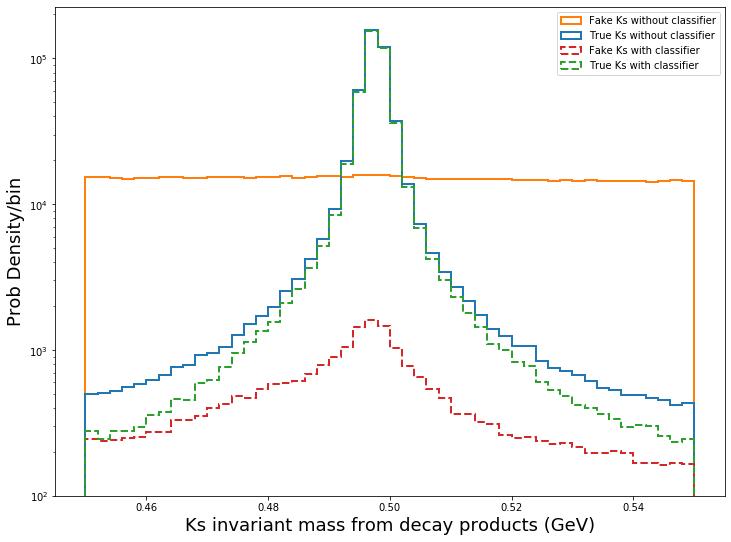
\includegraphics[width=0.8\linewidth]{kscutM}
	\caption{$K_S^0$ purity improvement with cut value of FBDT\_Ks at 0.74 applied. Blue solid line is true $K_S^0$ before KsFinder and green dashed line is the true $K_S^0$ after. The orange solid line is fake $K_S^0$ before KsFinder and red dashed line is fake $K_S^0$ after. 95.3\% of true $K_S^0$ are kept while 97.6\% the fake are rejected by the classification. }
\end{figure}

\subsection{Data Validation for Classifier}
The results from MC studies show an excellentperformance of KsFinder. However, such classification is based on the observables reconstructed from MC samples, and FastBDT algorithm is depending on the training features apparently. As a result, the validation of such tool on the real experiment data is necessary. This would justify the usage of classifier on data and is also essentially helpful to check the potential discrepancy between MC and data. 

The validation comes from the following aspects. First of all, since there's no ``isSignal" truth in real data, there's no way to direct check performance on data. Since the FastBDT method is based on the distribution of training variables, if these variables shows close distribution among MC and data, then the classification performance is expected to be close.

 Thus, variables must be compared between data and MC to ensure the consistence. Then, the expected performance represented by the distribution of selected $K_S^0$ should be similar between data and MC. Particularly, since $K_S^0$ candidates will be used for further reconstruction of $B^0$, its kinematics such mass and momentum may change after the classifier application, so the validation that approves no clear bias on $B^0$'s $M_{bc}$ and $\Delta E$ which are used for $B^0$ reconstruction is also needed.

We take the small data sample from Belle II early phase 3 operation experiment 7 and 8 in 2019 for comparison. The integral luminosity at $\Upsilon(4S)$ resonance is about 5.17 $\text{fb}^{-1}$.  MC13 sample is extracted from generic $B^0$ decay with equivalent events number. There are two campaigns of MC included (MC12b and MC13, later one is the latest). Fig 3-16 shows the invariant mass and momentum distributions from data and MC samples, and full comparison of all training variables is included in Appendix B. Most of the distribution shows a good consistence before and after using KsFinder. It shows that kinematics of $K_S^0$ in data and MC yield fairly close distributions and no clear bias is seen by applying the KsFinder cut.

\begin{figure}[H]
	\begin{subfigure}{0.5\linewidth}
		\includegraphics[page=2,height=4cm]{dataVarsPlot_Ks.pdf}
	\end{subfigure}
	\begin{subfigure}{0.5\linewidth}
		\includegraphics[page=7,height=4cm]{dataVarsPlot_Ks.pdf}
	\end{subfigure}
	\bigskip
	\begin{subfigure}{0.5\linewidth}
		\includegraphics[page=8,height=4cm]{dataVarsPlot_Ks.pdf}
	\end{subfigure}
	\begin{subfigure}{0.5\linewidth}
		\includegraphics[page=9,height=4cm]{dataVarsPlot_Ks.pdf}
	\end{subfigure}
\caption{The distribution of invariant mass from daughters and the momentum of x,y,z direction. Blue bar is from all MC13, cyan bar is the true $K_S^0$ in it. Yellow step histogram is data with no cut, solid red data with MC13 trained cut, and the dashed is with MC12b cut. Experimental data has a good agreement with MC before and after applying the KsFinder.}
\end{figure}

\subsection{KsFinder Effects on Kinematics Evaluation}
Implementing KsFinder for $K_S^0$ may induce extra bias on the event numbers for $K_S^0$. It's not easy to direct evaluate the impact of each variables in training towards the final signal yield because the output is non-linear dependence on those variables. However, we can directly use the output of KsFinder and introduce the scale factor when check the data and MC signal yields. 
 
A fit on invariant mass $M$ of $K_S^0$ candidates after varied cut on KsFinder output is done by modeling signal shape as double-Gaussian and background as Chebyshev polynomial. Significance is define as $S_{data/MC} = N_{signal} /N_total$ in data and MC from fitting using RooFit. A list of intervals of cut value on KsFinder output is made and the significance is calculated within each interval. Fitting results are shown in Fig 3.17 using loose and tight cut respectively. The fit plots in all cut intervals are included in Appendix C.  Data/MC correction is defined as:

\begin{equation}
	R = \frac{S_{MC}}{S_{data}}
\end{equation}



\begin{figure}[htpb]
	\begin{subfigure}{0.5\linewidth}
		\caption{Data,cut=0.2}
		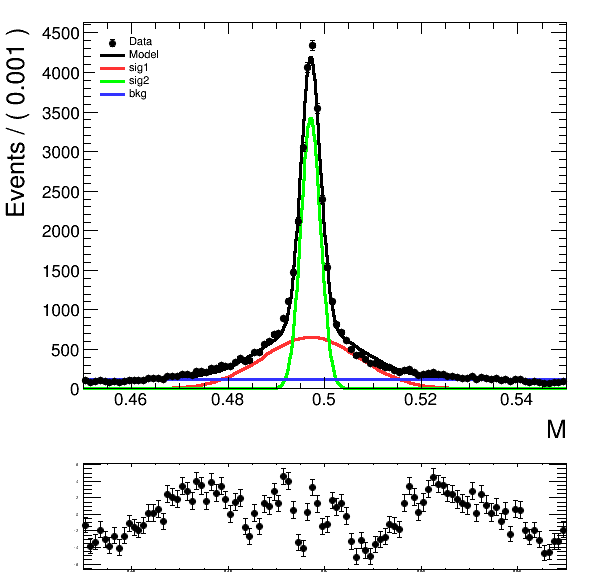
\includegraphics[width=1\linewidth]{ksDatamva0.2.png}
	\end{subfigure}
\begin{subfigure}{0.5\linewidth}
	\caption{MC,cut=0.2}
	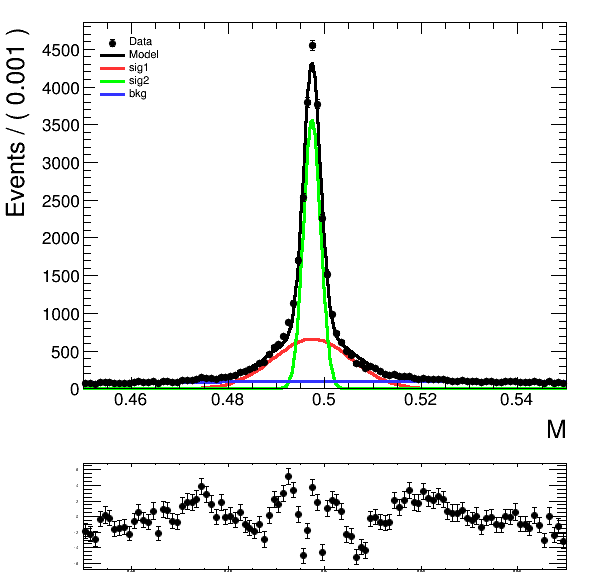
\includegraphics[width=1\linewidth]{ksMCmva0.2.png}
\end{subfigure}

\begin{subfigure}{0.5\linewidth}
	\caption{Data,cut=0.9}
	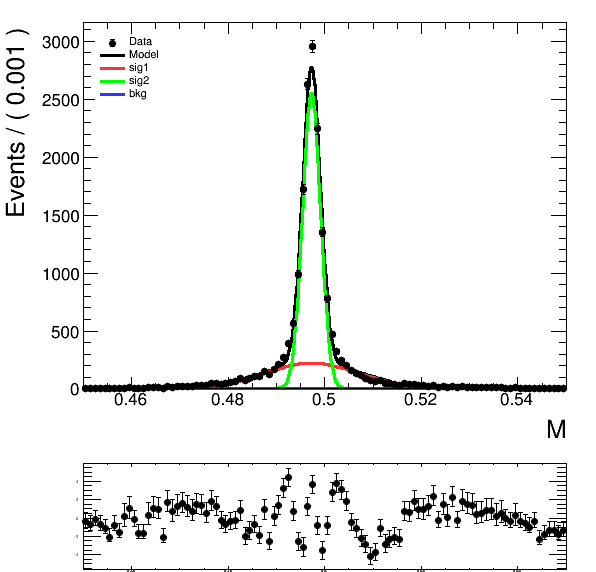
\includegraphics[width=1\linewidth]{ksDatamva0.9.png}
\end{subfigure}
\begin{subfigure}{0.5\linewidth}
	\caption{MC,cut=0.9}
	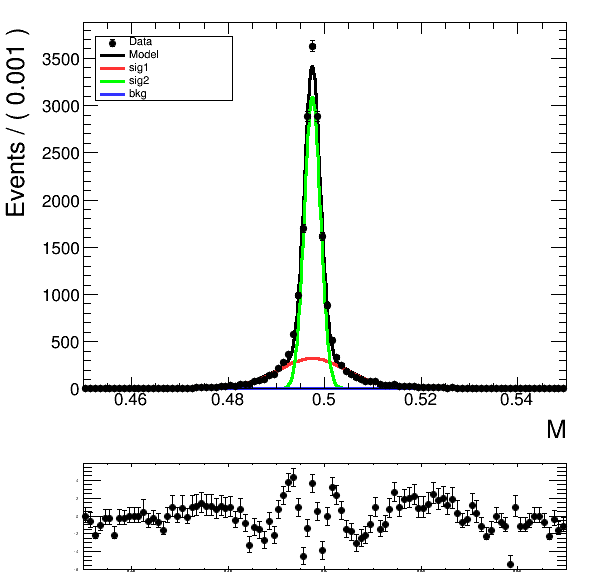
\includegraphics[width=1\linewidth]{ksMCmva0.9.png}
\end{subfigure}
\caption{Invariant mass fit of $K_S^0$ using cut at 0.2(loose) and 0.9(tight) to calculate $S_{data/MC}$.}
\end{figure}

The correction is defined by taking the R value within the chosen interval. Uncertainty of R is defined by the difference of maximum and minimum of R in all intervals. R is distributed as: 
\begin{figure}[H]
	\centering 
	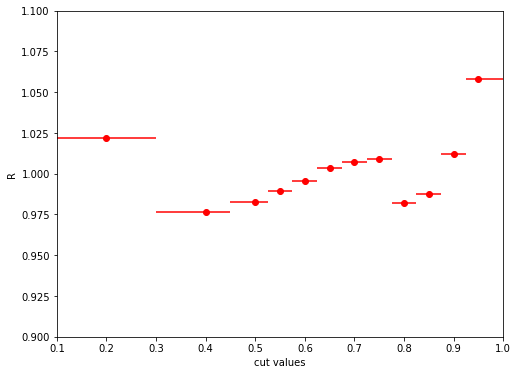
\includegraphics[width=0.7\linewidth]{Rc}
	\caption{Data MC correction induced by $K_S^0$ classifier.}
\end{figure}

The R, for example in cut value 0.74 of maximum FOM, is $R = 1.009\pm 0.081$. In $B^0 \to K_S^0  K_S^0  K_S^0$, the correction of $B^0$ events should be proportional to R to the three.  Correction that is implemented for $B^0$ is $1.027^{+0.33}_{-0.18}$. In most of the cut intervals, the R is within 2.5\% so the bias on $K_S^0$ numbers is very small.
\subsection{Summary}
The development of Belle II $K_S^0$ classifier is enlighten by the experience from Belle. A comprehensive study of training observables from $K_S^0$ decay characteristics has been exploited. It takes the advantage of FastBDT algorithm to achieve a high fake rejection power. As a result, classifier is able to give a output which can be used as a cut to select good $K_S^0$ candidates with high purity. The classifier is validated with real experimental data as well. A primary data validation study of KsFinder is conducted with implementing correction on data and MC along with its contribution to $B^0$. The performance of KsFinder is in a good shape and no clear bias is found on the yield of the number of $K_S^0$. For the reconstruction of $B^0 \to K_S^0  K_S^0  K_S^0$, the development of KsFinder is critical to suppress large fraction of combination background from fake $K_S^0$.

